\documentclass[1p]{elsarticle_modified}
%\bibliographystyle{elsarticle-num}

%\usepackage[colorlinks]{hyperref}
%\usepackage{abbrmath_seonhwa} %\Abb, \Ascr, \Acal ,\Abf, \Afrak
\usepackage{amsfonts}
\usepackage{amssymb}
\usepackage{amsmath}
\usepackage{amsthm}
\usepackage{scalefnt}
\usepackage{amsbsy}
\usepackage{kotex}
\usepackage{caption}
\usepackage{subfig}
\usepackage{color}
\usepackage{graphicx}
\usepackage{xcolor} %% white, black, red, green, blue, cyan, magenta, yellow
\usepackage{float}
\usepackage{setspace}
\usepackage{hyperref}

\usepackage{tikz}
\usetikzlibrary{arrows}

\usepackage{multirow}
\usepackage{array} % fixed length table
\usepackage{hhline}

%%%%%%%%%%%%%%%%%%%%%
\makeatletter
\renewcommand*\env@matrix[1][\arraystretch]{%
	\edef\arraystretch{#1}%
	\hskip -\arraycolsep
	\let\@ifnextchar\new@ifnextchar
	\array{*\c@MaxMatrixCols c}}
\makeatother %https://tex.stackexchange.com/questions/14071/how-can-i-increase-the-line-spacing-in-a-matrix
%%%%%%%%%%%%%%%

\usepackage[normalem]{ulem}

\newcommand{\msout}[1]{\ifmmode\text{\sout{\ensuremath{#1}}}\else\sout{#1}\fi}
%SOURCE: \msout is \stkout macro in https://tex.stackexchange.com/questions/20609/strikeout-in-math-mode

\newcommand{\cancel}[1]{
	\ifmmode
	{\color{red}\msout{#1}}
	\else
	{\color{red}\sout{#1}}
	\fi
}

\newcommand{\add}[1]{
	{\color{blue}\uwave{#1}}
}

\newcommand{\replace}[2]{
	\ifmmode
	{\color{red}\msout{#1}}{\color{blue}\uwave{#2}}
	\else
	{\color{red}\sout{#1}}{\color{blue}\uwave{#2}}
	\fi
}

\newcommand{\Sol}{\mathcal{S}} %segment
\newcommand{\D}{D} %diagram
\newcommand{\A}{\mathcal{A}} %arc


%%%%%%%%%%%%%%%%%%%%%%%%%%%%%5 test

\def\sl{\operatorname{\textup{SL}}(2,\Cbb)}
\def\psl{\operatorname{\textup{PSL}}(2,\Cbb)}
\def\quan{\mkern 1mu \triangleright \mkern 1mu}

\theoremstyle{definition}
\newtheorem{thm}{Theorem}[section]
\newtheorem{prop}[thm]{Proposition}
\newtheorem{lem}[thm]{Lemma}
\newtheorem{ques}[thm]{Question}
\newtheorem{cor}[thm]{Corollary}
\newtheorem{defn}[thm]{Definition}
\newtheorem{exam}[thm]{Example}
\newtheorem{rmk}[thm]{Remark}
\newtheorem{alg}[thm]{Algorithm}

\newcommand{\I}{\sqrt{-1}}
\begin{document}

%\begin{frontmatter}
%
%\title{Boundary parabolic representations of knots up to 8 crossings}
%
%%% Group authors per affiliation:
%\author{Yunhi Cho} 
%\address{Department of Mathematics, University of Seoul, Seoul, Korea}
%\ead{yhcho@uos.ac.kr}
%
%
%\author{Seonhwa Kim} %\fnref{s_kim}}
%\address{Center for Geometry and Physics, Institute for Basic Science, Pohang, 37673, Korea}
%\ead{ryeona17@ibs.re.kr}
%
%\author{Hyuk Kim}
%\address{Department of Mathematical Sciences, Seoul National University, Seoul 08826, Korea}
%\ead{hyukkim@snu.ac.kr}
%
%\author{Seokbeom Yoon}
%\address{Department of Mathematical Sciences, Seoul National University, Seoul, 08826,  Korea}
%\ead{sbyoon15@snu.ac.kr}
%
%\begin{abstract}
%We find all boundary parabolic representation of knots up to 8 crossings.
%
%\end{abstract}
%\begin{keyword}
%    \MSC[2010] 57M25 
%\end{keyword}
%
%\end{frontmatter}

%\linenumbers
%\tableofcontents
%
\newcommand\colored[1]{\textcolor{white}{\rule[-0.35ex]{0.8em}{1.4ex}}\kern-0.8em\color{red} #1}%
%\newcommand\colored[1]{\textcolor{white}{ #1}\kern-2.17ex	\textcolor{white}{ #1}\kern-1.81ex	\textcolor{white}{ #1}\kern-2.15ex\color{red}#1	}

{\Large $\underline{12n_{0728}~(K12n_{0728})}$}

\setlength{\tabcolsep}{10pt}
\renewcommand{\arraystretch}{1.6}
\vspace{1cm}\begin{tabular}{m{100pt}>{\centering\arraybackslash}m{274pt}}
\multirow{5}{120pt}{
	\centering
	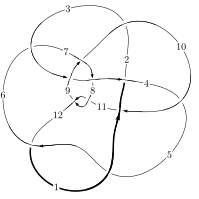
\includegraphics[width=112pt]{../../../GIT/diagram.site/Diagrams/png/2817_12n_0728.png}\\
\ \ \ A knot diagram\footnotemark}&
\allowdisplaybreaks
\textbf{Linearized knot diagam} \\
\cline{2-2}
 &
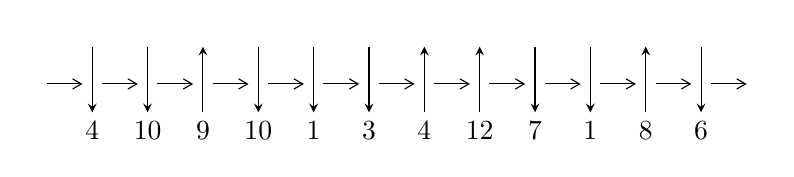
\begin{tikzpicture}[x=20pt, y=17pt]
	% nodes
	\node (C0) at (0, 0) {};
	\node (C1) at (1, 0) {};
	\node (C1U) at (1, +1) {};
	\node (C1D) at (1, -1) {4};

	\node (C2) at (2, 0) {};
	\node (C2U) at (2, +1) {};
	\node (C2D) at (2, -1) {10};

	\node (C3) at (3, 0) {};
	\node (C3U) at (3, +1) {};
	\node (C3D) at (3, -1) {9};

	\node (C4) at (4, 0) {};
	\node (C4U) at (4, +1) {};
	\node (C4D) at (4, -1) {10};

	\node (C5) at (5, 0) {};
	\node (C5U) at (5, +1) {};
	\node (C5D) at (5, -1) {1};

	\node (C6) at (6, 0) {};
	\node (C6U) at (6, +1) {};
	\node (C6D) at (6, -1) {3};

	\node (C7) at (7, 0) {};
	\node (C7U) at (7, +1) {};
	\node (C7D) at (7, -1) {4};

	\node (C8) at (8, 0) {};
	\node (C8U) at (8, +1) {};
	\node (C8D) at (8, -1) {12};

	\node (C9) at (9, 0) {};
	\node (C9U) at (9, +1) {};
	\node (C9D) at (9, -1) {7};

	\node (C10) at (10, 0) {};
	\node (C10U) at (10, +1) {};
	\node (C10D) at (10, -1) {1};

	\node (C11) at (11, 0) {};
	\node (C11U) at (11, +1) {};
	\node (C11D) at (11, -1) {8};

	\node (C12) at (12, 0) {};
	\node (C12U) at (12, +1) {};
	\node (C12D) at (12, -1) {6};
	\node (C13) at (13, 0) {};

	% arrows
	\draw[->,>={angle 60}]
	(C0) edge (C1) (C1) edge (C2) (C2) edge (C3) (C3) edge (C4) (C4) edge (C5) (C5) edge (C6) (C6) edge (C7) (C7) edge (C8) (C8) edge (C9) (C9) edge (C10) (C10) edge (C11) (C11) edge (C12) (C12) edge (C13) ;	\draw[->,>=stealth]
	(C1U) edge (C1D) (C2U) edge (C2D) (C3D) edge (C3U) (C4U) edge (C4D) (C5U) edge (C5D) (C6U) edge (C6D) (C7D) edge (C7U) (C8D) edge (C8U) (C9U) edge (C9D) (C10U) edge (C10D) (C11D) edge (C11U) (C12U) edge (C12D) ;
	\end{tikzpicture} \\
\hhline{~~} \\& 
\textbf{Solving Sequence} \\ \cline{2-2} 
 &
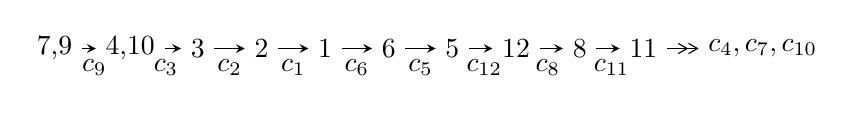
\begin{tikzpicture}[x=23pt, y=7pt]
	% node
	\node (A0) at (-1/8, 0) {7,9};
	\node (A1) at (17/16, 0) {4,10};
	\node (A2) at (17/8, 0) {3};
	\node (A3) at (25/8, 0) {2};
	\node (A4) at (33/8, 0) {1};
	\node (A5) at (41/8, 0) {6};
	\node (A6) at (49/8, 0) {5};
	\node (A7) at (57/8, 0) {12};
	\node (A8) at (65/8, 0) {8};
	\node (A9) at (73/8, 0) {11};
	\node (C1) at (1/2, -1) {$c_{9}$};
	\node (C2) at (13/8, -1) {$c_{3}$};
	\node (C3) at (21/8, -1) {$c_{2}$};
	\node (C4) at (29/8, -1) {$c_{1}$};
	\node (C5) at (37/8, -1) {$c_{6}$};
	\node (C6) at (45/8, -1) {$c_{5}$};
	\node (C7) at (53/8, -1) {$c_{12}$};
	\node (C8) at (61/8, -1) {$c_{8}$};
	\node (C9) at (69/8, -1) {$c_{11}$};
	\node (A10) at (11, 0) {$c_{4},c_{7},c_{10}$};

	% edge
	\draw[->,>=stealth]	
	(A0) edge (A1) (A1) edge (A2) (A2) edge (A3) (A3) edge (A4) (A4) edge (A5) (A5) edge (A6) (A6) edge (A7) (A7) edge (A8) (A8) edge (A9) ;
	\draw[->>,>={angle 60}]	
	(A9) edge (A10);
\end{tikzpicture} \\ 

\end{tabular} \\

\footnotetext{
The image of knot diagram is generated by the software ``\textbf{Draw programme}" developed by Andrew Bartholomew(\url{http://www.layer8.co.uk/maths/draw/index.htm\#Running-draw}), where we modified some parts for our purpose(\url{https://github.com/CATsTAILs/LinksPainter}).
}\phantom \\ \newline 
\centering \textbf{Ideals for irreducible components\footnotemark of $X_{\text{par}}$} 
 
\begin{align*}
I^u_{1}&=\langle 
-1.01387\times10^{267} u^{81}+3.48609\times10^{267} u^{80}+\cdots+2.22405\times10^{267} b+4.23115\times10^{269},\\
\phantom{I^u_{1}}&\phantom{= \langle  }-2.64646\times10^{270} u^{81}+8.98482\times10^{270} u^{80}+\cdots+1.75700\times10^{269} a+1.03533\times10^{273},\\
\phantom{I^u_{1}}&\phantom{= \langle  }u^{82}-4 u^{81}+\cdots-894 u+237\rangle \\
I^u_{2}&=\langle 
-5.22864\times10^{27} u^{28}-2.99746\times10^{31} u^{27}+\cdots+1.50231\times10^{32} b-4.81229\times10^{32},\\
\phantom{I^u_{2}}&\phantom{= \langle  }-1.28844\times10^{32} u^{28}-5.79283\times10^{31} u^{27}+\cdots+5.00769\times10^{31} a-4.89974\times10^{32},\;u^{29}+u^{28}+\cdots+21 u+3\rangle \\
\\
\end{align*}
\raggedright * 2 irreducible components of $\dim_{\mathbb{C}}=0$, with total 111 representations.\\
\footnotetext{All coefficients of polynomials are rational numbers. But the coefficients are sometimes approximated in decimal forms when there is not enough margin.}
\newpage
\renewcommand{\arraystretch}{1}
\centering \section*{I. $I^u_{1}= \langle -1.01\times10^{267} u^{81}+3.49\times10^{267} u^{80}+\cdots+2.22\times10^{267} b+4.23\times10^{269},\;-2.65\times10^{270} u^{81}+8.98\times10^{270} u^{80}+\cdots+1.76\times10^{269} a+1.04\times10^{273},\;u^{82}-4 u^{81}+\cdots-894 u+237 \rangle$}
\flushleft \textbf{(i) Arc colorings}\\
\begin{tabular}{m{7pt} m{180pt} m{7pt} m{180pt} }
\flushright $a_{7}=$&$\begin{pmatrix}0\\u\end{pmatrix}$ \\
\flushright $a_{9}=$&$\begin{pmatrix}1\\0\end{pmatrix}$ \\
\flushright $a_{4}=$&$\begin{pmatrix}15.0624 u^{81}-51.1374 u^{80}+\cdots+12694.4 u-5892.60\\0.455867 u^{81}-1.56745 u^{80}+\cdots+424.525 u-190.246\end{pmatrix}$ \\
\flushright $a_{10}=$&$\begin{pmatrix}1\\u^2\end{pmatrix}$ \\
\flushright $a_{3}=$&$\begin{pmatrix}14.6066 u^{81}-49.5699 u^{80}+\cdots+12269.8 u-5702.36\\0.455867 u^{81}-1.56745 u^{80}+\cdots+424.525 u-190.246\end{pmatrix}$ \\
\flushright $a_{2}=$&$\begin{pmatrix}9.68886 u^{81}-32.9414 u^{80}+\cdots+8238.54 u-3793.65\\-1.52253 u^{81}+5.00949 u^{80}+\cdots-1129.77 u+530.774\end{pmatrix}$ \\
\flushright $a_{1}=$&$\begin{pmatrix}-9.32638 u^{81}+30.9392 u^{80}+\cdots-7468.80 u+3517.86\\0.580835 u^{81}-1.94165 u^{80}+\cdots+527.411 u-163.415\end{pmatrix}$ \\
\flushright $a_{6}=$&$\begin{pmatrix}-10.4342 u^{81}+34.5042 u^{80}+\cdots-8588.49 u+3567.69\\-0.0359770 u^{81}+0.402833 u^{80}+\cdots-246.388 u+125.616\end{pmatrix}$ \\
\flushright $a_{5}=$&$\begin{pmatrix}20.0850 u^{81}-68.1817 u^{80}+\cdots+16846.5 u-7861.99\\2.37573 u^{81}-8.00559 u^{80}+\cdots+1957.35 u-912.163\end{pmatrix}$ \\
\flushright $a_{12}=$&$\begin{pmatrix}-44.6363 u^{81}+148.888 u^{80}+\cdots-36104.8 u+16270.5\\-0.966828 u^{81}+3.01023 u^{80}+\cdots-682.104 u+297.723\end{pmatrix}$ \\
\flushright $a_{8}=$&$\begin{pmatrix}-11.1285 u^{81}+37.2025 u^{80}+\cdots-9471.64 u+3960.48\\-0.658286 u^{81}+2.29544 u^{80}+\cdots-634.762 u+267.171\end{pmatrix}$ \\
\flushright $a_{11}=$&$\begin{pmatrix}-44.4234 u^{81}+146.964 u^{80}+\cdots-35127.7 u+15332.5\\-3.66095 u^{81}+11.6545 u^{80}+\cdots-2709.62 u+1037.57\end{pmatrix}$\\&\end{tabular}
\flushleft \textbf{(ii) Obstruction class $= -1$}\\~\\
\flushleft \textbf{(iii) Cusp Shapes $= 154.575 u^{81}-514.077 u^{80}+\cdots+124681. u-53829.8$}\\~\\
\newpage\renewcommand{\arraystretch}{1}
\flushleft \textbf{(iv) u-Polynomials at the component}\newline \\
\begin{tabular}{m{50pt}|m{274pt}}
Crossings & \hspace{64pt}u-Polynomials at each crossing \\
\hline $$\begin{aligned}c_{1}\end{aligned}$$&$\begin{aligned}
&u^{82}+14 u^{81}+\cdots-99113733 u+12092767
\end{aligned}$\\
\hline $$\begin{aligned}c_{2}\end{aligned}$$&$\begin{aligned}
&3(3 u^{82}+12 u^{81}+\cdots+1.10464\times10^{9} u-1.02450\times10^{8})
\end{aligned}$\\
\hline $$\begin{aligned}c_{3}\end{aligned}$$&$\begin{aligned}
&3(3 u^{82}+3 u^{81}+\cdots+7 u+1)
\end{aligned}$\\
\hline $$\begin{aligned}c_{4}\end{aligned}$$&$\begin{aligned}
&3(3 u^{82}-140 u^{80}+\cdots-10653 u-4399)
\end{aligned}$\\
\hline $$\begin{aligned}c_{5},c_{12}\end{aligned}$$&$\begin{aligned}
&u^{82}+10 u^{80}+\cdots-1416 u-528
\end{aligned}$\\
\hline $$\begin{aligned}c_{6}\end{aligned}$$&$\begin{aligned}
&u^{82}+2 u^{81}+\cdots+29 u-47
\end{aligned}$\\
\hline $$\begin{aligned}c_{7}\end{aligned}$$&$\begin{aligned}
&u^{82}+23 u^{80}+\cdots-84216 u-19056
\end{aligned}$\\
\hline $$\begin{aligned}c_{8},c_{11}\end{aligned}$$&$\begin{aligned}
&u^{82}+2 u^{81}+\cdots+169 u-97
\end{aligned}$\\
\hline $$\begin{aligned}c_{9}\end{aligned}$$&$\begin{aligned}
&u^{82}-4 u^{81}+\cdots-894 u+237
\end{aligned}$\\
\hline $$\begin{aligned}c_{10}\end{aligned}$$&$\begin{aligned}
&u^{82}-3 u^{81}+\cdots+5918619 u-282651
\end{aligned}$\\
\hline
\end{tabular}\\~\\
\newpage\renewcommand{\arraystretch}{1}
\flushleft \textbf{(v) Riley Polynomials at the component}\newline \\
\begin{tabular}{m{50pt}|m{274pt}}
Crossings & \hspace{64pt}Riley Polynomials at each crossing \\
\hline $$\begin{aligned}c_{1}\end{aligned}$$&$\begin{aligned}
&y^{82}-126 y^{81}+\cdots-2530004844652363 y+146235013716289
\end{aligned}$\\
\hline $$\begin{aligned}c_{2}\end{aligned}$$&$\begin{aligned}
&9\\
&\cdot(9 y^{82}-390 y^{81}+\cdots-204245228366900018 y+10495960905341209)
\end{aligned}$\\
\hline $$\begin{aligned}c_{3}\end{aligned}$$&$\begin{aligned}
&9(9 y^{82}+123 y^{81}+\cdots-27 y+1)
\end{aligned}$\\
\hline $$\begin{aligned}c_{4}\end{aligned}$$&$\begin{aligned}
&9(9 y^{82}-840 y^{81}+\cdots-1.02859\times10^{7} y+1.93512\times10^{7})
\end{aligned}$\\
\hline $$\begin{aligned}c_{5},c_{12}\end{aligned}$$&$\begin{aligned}
&y^{82}+20 y^{81}+\cdots-716736 y+278784
\end{aligned}$\\
\hline $$\begin{aligned}c_{6}\end{aligned}$$&$\begin{aligned}
&y^{82}-8 y^{81}+\cdots-9959 y+2209
\end{aligned}$\\
\hline $$\begin{aligned}c_{7}\end{aligned}$$&$\begin{aligned}
&y^{82}+46 y^{81}+\cdots+23494984512 y+363131136
\end{aligned}$\\
\hline $$\begin{aligned}c_{8},c_{11}\end{aligned}$$&$\begin{aligned}
&y^{82}-28 y^{81}+\cdots-256511 y+9409
\end{aligned}$\\
\hline $$\begin{aligned}c_{9}\end{aligned}$$&$\begin{aligned}
&y^{82}-12 y^{81}+\cdots-2374338 y+56169
\end{aligned}$\\
\hline $$\begin{aligned}c_{10}\end{aligned}$$&$\begin{aligned}
&y^{82}-111 y^{81}+\cdots-288406262487 y+79891587801
\end{aligned}$\\
\hline
\end{tabular}\\~\\
\newpage\flushleft \textbf{(vi) Complex Volumes and Cusp Shapes}
$$\begin{array}{c|c|c}  
\text{Solutions to }I^u_{1}& \I (\text{vol} + \sqrt{-1}CS) & \text{Cusp shape}\\
 \hline 
\begin{aligned}
u &= -0.850271 + 0.515578 I \\
a &= \phantom{-}0.271447 - 0.749585 I \\
b &= \phantom{-}1.179440 - 0.554371 I\end{aligned}
 & -7.33455 + 2.04069 I & \phantom{-0.000000 } 0 \\ \hline\begin{aligned}
u &= -0.850271 - 0.515578 I \\
a &= \phantom{-}0.271447 + 0.749585 I \\
b &= \phantom{-}1.179440 + 0.554371 I\end{aligned}
 & -7.33455 - 2.04069 I & \phantom{-0.000000 } 0 \\ \hline\begin{aligned}
u &= -0.755219 + 0.688817 I \\
a &= -0.72036 + 1.59123 I \\
b &= \phantom{-}0.701325 + 0.987821 I\end{aligned}
 & \phantom{-}1.00223 + 2.76606 I & \phantom{-0.000000 } 0 \\ \hline\begin{aligned}
u &= -0.755219 - 0.688817 I \\
a &= -0.72036 - 1.59123 I \\
b &= \phantom{-}0.701325 - 0.987821 I\end{aligned}
 & \phantom{-}1.00223 - 2.76606 I & \phantom{-0.000000 } 0 \\ \hline\begin{aligned}
u &= -0.398931 + 0.892202 I \\
a &= \phantom{-}0.834745 - 0.074502 I \\
b &= -0.743019 - 0.751372 I\end{aligned}
 & \phantom{-}4.58774 + 5.09155 I & \phantom{-0.000000 } 0 \\ \hline\begin{aligned}
u &= -0.398931 - 0.892202 I \\
a &= \phantom{-}0.834745 + 0.074502 I \\
b &= -0.743019 + 0.751372 I\end{aligned}
 & \phantom{-}4.58774 - 5.09155 I & \phantom{-0.000000 } 0 \\ \hline\begin{aligned}
u &= \phantom{-}0.645792 + 0.799973 I \\
a &= \phantom{-}0.285156 + 0.007683 I \\
b &= \phantom{-}0.588642 + 0.643448 I\end{aligned}
 & \phantom{-}1.69738 + 2.28323 I & \phantom{-0.000000 } 0 \\ \hline\begin{aligned}
u &= \phantom{-}0.645792 - 0.799973 I \\
a &= \phantom{-}0.285156 - 0.007683 I \\
b &= \phantom{-}0.588642 - 0.643448 I\end{aligned}
 & \phantom{-}1.69738 - 2.28323 I & \phantom{-0.000000 } 0 \\ \hline\begin{aligned}
u &= -0.751624 + 0.604004 I \\
a &= \phantom{-}0.18526 - 2.11592 I \\
b &= -0.297311 - 0.628227 I\end{aligned}
 & -6.95730 + 2.32221 I & \phantom{-0.000000 } 0 \\ \hline\begin{aligned}
u &= -0.751624 - 0.604004 I \\
a &= \phantom{-}0.18526 + 2.11592 I \\
b &= -0.297311 + 0.628227 I\end{aligned}
 & -6.95730 - 2.32221 I & \phantom{-0.000000 } 0\\
 \hline 
 \end{array}$$\newpage$$\begin{array}{c|c|c}  
\text{Solutions to }I^u_{1}& \I (\text{vol} + \sqrt{-1}CS) & \text{Cusp shape}\\
 \hline 
\begin{aligned}
u &= -0.927322 + 0.255571 I \\
a &= -0.154516 + 0.769316 I \\
b &= -0.320781 + 1.056570 I\end{aligned}
 & -0.09944 + 1.66245 I & \phantom{-0.000000 } 0 \\ \hline\begin{aligned}
u &= -0.927322 - 0.255571 I \\
a &= -0.154516 - 0.769316 I \\
b &= -0.320781 - 1.056570 I\end{aligned}
 & -0.09944 - 1.66245 I & \phantom{-0.000000 } 0 \\ \hline\begin{aligned}
u &= \phantom{-}0.887925 + 0.302340 I \\
a &= -0.299354 - 0.748760 I \\
b &= -1.58756 - 0.77790 I\end{aligned}
 & -6.61377 + 4.10167 I & \phantom{-0.000000 } 0 \\ \hline\begin{aligned}
u &= \phantom{-}0.887925 - 0.302340 I \\
a &= -0.299354 + 0.748760 I \\
b &= -1.58756 + 0.77790 I\end{aligned}
 & -6.61377 - 4.10167 I & \phantom{-0.000000 } 0 \\ \hline\begin{aligned}
u &= \phantom{-}0.700572 + 0.798714 I \\
a &= \phantom{-}0.577755 - 0.588155 I \\
b &= \phantom{-}1.338410 - 0.294958 I\end{aligned}
 & \phantom{-}4.41321 + 0.49327 I & \phantom{-0.000000 } 0 \\ \hline\begin{aligned}
u &= \phantom{-}0.700572 - 0.798714 I \\
a &= \phantom{-}0.577755 + 0.588155 I \\
b &= \phantom{-}1.338410 + 0.294958 I\end{aligned}
 & \phantom{-}4.41321 - 0.49327 I & \phantom{-0.000000 } 0 \\ \hline\begin{aligned}
u &= -0.819668 + 0.376320 I \\
a &= -0.468203 + 1.175900 I \\
b &= -1.33128 + 1.44116 I\end{aligned}
 & -6.30926 + 8.22313 I & \phantom{-0.000000 } 0 \\ \hline\begin{aligned}
u &= -0.819668 - 0.376320 I \\
a &= -0.468203 - 1.175900 I \\
b &= -1.33128 - 1.44116 I\end{aligned}
 & -6.30926 - 8.22313 I & \phantom{-0.000000 } 0 \\ \hline\begin{aligned}
u &= \phantom{-}0.794993 + 0.390347 I \\
a &= -0.155542 - 1.291390 I \\
b &= \phantom{-}1.24485 - 1.06941 I\end{aligned}
 & \phantom{-}1.85456 - 6.66524 I & \phantom{-0.000000 } 0 \\ \hline\begin{aligned}
u &= \phantom{-}0.794993 - 0.390347 I \\
a &= -0.155542 + 1.291390 I \\
b &= \phantom{-}1.24485 + 1.06941 I\end{aligned}
 & \phantom{-}1.85456 + 6.66524 I & \phantom{-0.000000 } 0\\
 \hline 
 \end{array}$$\newpage$$\begin{array}{c|c|c}  
\text{Solutions to }I^u_{1}& \I (\text{vol} + \sqrt{-1}CS) & \text{Cusp shape}\\
 \hline 
\begin{aligned}
u &= -0.992411 + 0.559301 I \\
a &= -0.256575 - 1.132100 I \\
b &= \phantom{-}0.109802 - 0.482795 I\end{aligned}
 & -6.97250 + 2.76431 I & \phantom{-0.000000 } 0 \\ \hline\begin{aligned}
u &= -0.992411 - 0.559301 I \\
a &= -0.256575 + 1.132100 I \\
b &= \phantom{-}0.109802 + 0.482795 I\end{aligned}
 & -6.97250 - 2.76431 I & \phantom{-0.000000 } 0 \\ \hline\begin{aligned}
u &= -1.016370 + 0.514652 I \\
a &= \phantom{-}0.113323 + 0.981555 I \\
b &= \phantom{-}0.442694 + 1.098610 I\end{aligned}
 & -0.307621 + 1.054850 I & \phantom{-0.000000 } 0 \\ \hline\begin{aligned}
u &= -1.016370 - 0.514652 I \\
a &= \phantom{-}0.113323 - 0.981555 I \\
b &= \phantom{-}0.442694 - 1.098610 I\end{aligned}
 & -0.307621 - 1.054850 I & \phantom{-0.000000 } 0 \\ \hline\begin{aligned}
u &= \phantom{-}0.783658 + 0.839527 I \\
a &= -0.232652 - 0.491677 I \\
b &= \phantom{-}1.088250 - 0.358012 I\end{aligned}
 & \phantom{-}5.64411 - 3.29713 I & \phantom{-0.000000 } 0 \\ \hline\begin{aligned}
u &= \phantom{-}0.783658 - 0.839527 I \\
a &= -0.232652 + 0.491677 I \\
b &= \phantom{-}1.088250 + 0.358012 I\end{aligned}
 & \phantom{-}5.64411 + 3.29713 I & \phantom{-0.000000 } 0 \\ \hline\begin{aligned}
u &= \phantom{-}0.772392 + 0.261309 I \\
a &= \phantom{-}0.23922 + 1.65529 I \\
b &= \phantom{-}0.92824 + 1.39853 I\end{aligned}
 & -8.69968 - 1.42199 I & \phantom{-0.000000 } 0 \\ \hline\begin{aligned}
u &= \phantom{-}0.772392 - 0.261309 I \\
a &= \phantom{-}0.23922 - 1.65529 I \\
b &= \phantom{-}0.92824 - 1.39853 I\end{aligned}
 & -8.69968 + 1.42199 I & \phantom{-0.000000 } 0 \\ \hline\begin{aligned}
u &= \phantom{-}0.754514 + 0.276947 I \\
a &= -0.32775 + 2.60121 I \\
b &= \phantom{-}0.080369 + 1.137500 I\end{aligned}
 & -8.60566 - 0.81317 I & \phantom{-0.000000 } 0 \\ \hline\begin{aligned}
u &= \phantom{-}0.754514 - 0.276947 I \\
a &= -0.32775 - 2.60121 I \\
b &= \phantom{-}0.080369 - 1.137500 I\end{aligned}
 & -8.60566 + 0.81317 I & \phantom{-0.000000 } 0\\
 \hline 
 \end{array}$$\newpage$$\begin{array}{c|c|c}  
\text{Solutions to }I^u_{1}& \I (\text{vol} + \sqrt{-1}CS) & \text{Cusp shape}\\
 \hline 
\begin{aligned}
u &= -0.653902 + 0.457863 I \\
a &= -0.091022 + 1.039930 I \\
b &= \phantom{-}0.248927 + 0.754353 I\end{aligned}
 & -0.301195 + 1.328750 I & \phantom{-0.000000 } 0 \\ \hline\begin{aligned}
u &= -0.653902 - 0.457863 I \\
a &= -0.091022 - 1.039930 I \\
b &= \phantom{-}0.248927 - 0.754353 I\end{aligned}
 & -0.301195 - 1.328750 I & \phantom{-0.000000 } 0 \\ \hline\begin{aligned}
u &= \phantom{-}0.778139\phantom{ +0.000000I} \\
a &= \phantom{-}2.71056\phantom{ +0.000000I} \\
b &= \phantom{-}0.253134\phantom{ +0.000000I}\end{aligned}
 & -2.10752\phantom{ +0.000000I} & \phantom{-0.000000 } 0 \\ \hline\begin{aligned}
u &= \phantom{-}0.986047 + 0.760457 I \\
a &= \phantom{-}0.246197 + 1.252340 I \\
b &= -0.990587 + 0.961519 I\end{aligned}
 & \phantom{-}0.85224 - 8.09504 I & \phantom{-0.000000 } 0 \\ \hline\begin{aligned}
u &= \phantom{-}0.986047 - 0.760457 I \\
a &= \phantom{-}0.246197 - 1.252340 I \\
b &= -0.990587 - 0.961519 I\end{aligned}
 & \phantom{-}0.85224 + 8.09504 I & \phantom{-0.000000 } 0 \\ \hline\begin{aligned}
u &= -0.694300 + 0.284103 I \\
a &= -1.35570 + 1.82174 I \\
b &= \phantom{-}0.138687 + 0.871125 I\end{aligned}
 & -0.65973 + 2.45836 I & \phantom{-0.000000 } 0 \\ \hline\begin{aligned}
u &= -0.694300 - 0.284103 I \\
a &= -1.35570 - 1.82174 I \\
b &= \phantom{-}0.138687 - 0.871125 I\end{aligned}
 & -0.65973 - 2.45836 I & \phantom{-0.000000 } 0 \\ \hline\begin{aligned}
u &= -0.644494 + 0.341367 I \\
a &= \phantom{-}0.17207 + 3.88745 I \\
b &= \phantom{-}0.274695 + 0.835596 I\end{aligned}
 & -5.69889 - 5.28203 I & \phantom{-0.000000 } 0 \\ \hline\begin{aligned}
u &= -0.644494 - 0.341367 I \\
a &= \phantom{-}0.17207 - 3.88745 I \\
b &= \phantom{-}0.274695 - 0.835596 I\end{aligned}
 & -5.69889 + 5.28203 I & \phantom{-0.000000 } 0 \\ \hline\begin{aligned}
u &= \phantom{-}0.578089 + 0.442723 I \\
a &= \phantom{-}0.52803 - 3.87108 I \\
b &= \phantom{-}0.466703 - 0.384771 I\end{aligned}
 & -5.38362 - 7.14150 I & \phantom{-0.000000 } 0\\
 \hline 
 \end{array}$$\newpage$$\begin{array}{c|c|c}  
\text{Solutions to }I^u_{1}& \I (\text{vol} + \sqrt{-1}CS) & \text{Cusp shape}\\
 \hline 
\begin{aligned}
u &= \phantom{-}0.578089 - 0.442723 I \\
a &= \phantom{-}0.52803 + 3.87108 I \\
b &= \phantom{-}0.466703 + 0.384771 I\end{aligned}
 & -5.38362 + 7.14150 I & \phantom{-0.000000 } 0 \\ \hline\begin{aligned}
u &= -0.993572 + 0.801631 I \\
a &= -0.198392 - 0.784097 I \\
b &= -0.981533 - 0.850677 I\end{aligned}
 & -1.73300 + 4.30022 I & \phantom{-0.000000 } 0 \\ \hline\begin{aligned}
u &= -0.993572 - 0.801631 I \\
a &= -0.198392 + 0.784097 I \\
b &= -0.981533 + 0.850677 I\end{aligned}
 & -1.73300 - 4.30022 I & \phantom{-0.000000 } 0 \\ \hline\begin{aligned}
u &= \phantom{-}0.969380 + 0.897508 I \\
a &= \phantom{-}0.214456 - 1.096160 I \\
b &= \phantom{-}1.18899 - 1.21639 I\end{aligned}
 & \phantom{-}1.74052 - 10.48820 I & \phantom{-0.000000 } 0 \\ \hline\begin{aligned}
u &= \phantom{-}0.969380 - 0.897508 I \\
a &= \phantom{-}0.214456 + 1.096160 I \\
b &= \phantom{-}1.18899 + 1.21639 I\end{aligned}
 & \phantom{-}1.74052 + 10.48820 I & \phantom{-0.000000 } 0 \\ \hline\begin{aligned}
u &= \phantom{-}0.571480 + 0.349378 I \\
a &= \phantom{-}0.162785 + 0.461752 I \\
b &= -1.46297 + 0.68408 I\end{aligned}
 & -0.550623 - 1.155750 I & \phantom{-0.000000 -}0. + 9.52354 I \\ \hline\begin{aligned}
u &= \phantom{-}0.571480 - 0.349378 I \\
a &= \phantom{-}0.162785 - 0.461752 I \\
b &= -1.46297 - 0.68408 I\end{aligned}
 & -0.550623 + 1.155750 I & \phantom{-0.000000 } 0. - 9.52354 I \\ \hline\begin{aligned}
u &= \phantom{-}0.646667 + 0.157930 I \\
a &= -1.86555 + 1.47666 I \\
b &= -0.445822 + 0.624782 I\end{aligned}
 & \phantom{-}2.08117 - 5.13424 I & \phantom{-0.000000 -}0. + 9.56633 I \\ \hline\begin{aligned}
u &= \phantom{-}0.646667 - 0.157930 I \\
a &= -1.86555 - 1.47666 I \\
b &= -0.445822 - 0.624782 I\end{aligned}
 & \phantom{-}2.08117 + 5.13424 I & \phantom{-0.000000 } 0. - 9.56633 I \\ \hline\begin{aligned}
u &= \phantom{-}1.096790 + 0.760066 I \\
a &= -0.469877 + 1.140750 I \\
b &= -1.048700 + 0.777334 I\end{aligned}
 & \phantom{-}3.17403 - 6.33099 I & \phantom{-0.000000 } 0\\
 \hline 
 \end{array}$$\newpage$$\begin{array}{c|c|c}  
\text{Solutions to }I^u_{1}& \I (\text{vol} + \sqrt{-1}CS) & \text{Cusp shape}\\
 \hline 
\begin{aligned}
u &= \phantom{-}1.096790 - 0.760066 I \\
a &= -0.469877 - 1.140750 I \\
b &= -1.048700 - 0.777334 I\end{aligned}
 & \phantom{-}3.17403 + 6.33099 I & \phantom{-0.000000 } 0 \\ \hline\begin{aligned}
u &= \phantom{-}0.665121\phantom{ +0.000000I} \\
a &= -3.00914\phantom{ +0.000000I} \\
b &= \phantom{-}0.299281\phantom{ +0.000000I}\end{aligned}
 & -9.80679\phantom{ +0.000000I} & -71.6570\phantom{ +0.000000I} \\ \hline\begin{aligned}
u &= -0.804129 + 1.139850 I \\
a &= -0.660591 + 0.539069 I \\
b &= \phantom{-}0.440518 + 0.824186 I\end{aligned}
 & \phantom{-}1.94276 + 5.50841 I & \phantom{-0.000000 } 0 \\ \hline\begin{aligned}
u &= -0.804129 - 1.139850 I \\
a &= -0.660591 - 0.539069 I \\
b &= \phantom{-}0.440518 - 0.824186 I\end{aligned}
 & \phantom{-}1.94276 - 5.50841 I & \phantom{-0.000000 } 0 \\ \hline\begin{aligned}
u &= \phantom{-}1.02823 + 0.99300 I \\
a &= -0.691003 + 0.097488 I \\
b &= -0.449010 - 0.350908 I\end{aligned}
 & \phantom{-}1.83592 + 3.56054 I & \phantom{-0.000000 } 0 \\ \hline\begin{aligned}
u &= \phantom{-}1.02823 - 0.99300 I \\
a &= -0.691003 - 0.097488 I \\
b &= -0.449010 + 0.350908 I\end{aligned}
 & \phantom{-}1.83592 - 3.56054 I & \phantom{-0.000000 } 0 \\ \hline\begin{aligned}
u &= \phantom{-}1.15815 + 0.85043 I \\
a &= \phantom{-}0.019191 + 0.727549 I \\
b &= -0.637514 + 0.265254 I\end{aligned}
 & \phantom{-}4.52317 - 2.87684 I & \phantom{-0.000000 } 0 \\ \hline\begin{aligned}
u &= \phantom{-}1.15815 - 0.85043 I \\
a &= \phantom{-}0.019191 - 0.727549 I \\
b &= -0.637514 - 0.265254 I\end{aligned}
 & \phantom{-}4.52317 + 2.87684 I & \phantom{-0.000000 } 0 \\ \hline\begin{aligned}
u &= -0.517394 + 0.218711 I \\
a &= \phantom{-}0.38948 - 2.40080 I \\
b &= -0.94523 - 1.19596 I\end{aligned}
 & \phantom{-}2.61465 + 0.77345 I & \phantom{-}                -6
1.138777 + 0. 10   I\phantom{ +0.000000I} \\ \hline\begin{aligned}
u &= -0.517394 - 0.218711 I \\
a &= \phantom{-}0.38948 + 2.40080 I \\
b &= -0.94523 + 1.19596 I\end{aligned}
 & \phantom{-}2.61465 - 0.77345 I & \phantom{-}                -6
1.138777 + 0. 10   I\phantom{ +0.000000I}\\
 \hline 
 \end{array}$$\newpage$$\begin{array}{c|c|c}  
\text{Solutions to }I^u_{1}& \I (\text{vol} + \sqrt{-1}CS) & \text{Cusp shape}\\
 \hline 
\begin{aligned}
u &= -0.387563 + 0.385990 I \\
a &= -0.655661 + 1.116930 I \\
b &= \phantom{-}0.23435 + 2.08764 I\end{aligned}
 & \phantom{-}0.416926 - 0.015506 I & -10.35701 + 0. I\phantom{ +0.000000I} \\ \hline\begin{aligned}
u &= -0.387563 - 0.385990 I \\
a &= -0.655661 - 1.116930 I \\
b &= \phantom{-}0.23435 - 2.08764 I\end{aligned}
 & \phantom{-}0.416926 + 0.015506 I & -10.35701 + 0. I\phantom{ +0.000000I} \\ \hline\begin{aligned}
u &= \phantom{-}0.525179 + 0.030642 I \\
a &= \phantom{-}1.98553 + 0.13237 I \\
b &= -0.219757 + 0.080532 I\end{aligned}
 & -1.54159 - 0.00262 I & -9.47854 - 0.67252 I \\ \hline\begin{aligned}
u &= \phantom{-}0.525179 - 0.030642 I \\
a &= \phantom{-}1.98553 - 0.13237 I \\
b &= -0.219757 - 0.080532 I\end{aligned}
 & -1.54159 + 0.00262 I & -9.47854 + 0.67252 I \\ \hline\begin{aligned}
u &= -1.08161 + 1.04076 I \\
a &= \phantom{-}0.249928 - 0.089307 I \\
b &= -0.223261 - 0.241635 I\end{aligned}
 & -0.92678 + 2.59995 I & \phantom{-0.000000 } 0 \\ \hline\begin{aligned}
u &= -1.08161 - 1.04076 I \\
a &= \phantom{-}0.249928 + 0.089307 I \\
b &= -0.223261 + 0.241635 I\end{aligned}
 & -0.92678 - 2.59995 I & \phantom{-0.000000 } 0 \\ \hline\begin{aligned}
u &= -1.27100 + 0.88966 I \\
a &= \phantom{-}0.140122 + 1.152840 I \\
b &= \phantom{-}1.08021 + 1.07345 I\end{aligned}
 & -8.25214 + 9.72918 I & \phantom{-0.000000 } 0 \\ \hline\begin{aligned}
u &= -1.27100 - 0.88966 I \\
a &= \phantom{-}0.140122 - 1.152840 I \\
b &= \phantom{-}1.08021 - 1.07345 I\end{aligned}
 & -8.25214 - 9.72918 I & \phantom{-0.000000 } 0 \\ \hline\begin{aligned}
u &= \phantom{-}1.23138 + 0.94766 I \\
a &= -0.005878 + 1.239660 I \\
b &= -1.12230 + 1.17955 I\end{aligned}
 & -6.4341 - 17.3813 I & \phantom{-0.000000 } 0 \\ \hline\begin{aligned}
u &= \phantom{-}1.23138 - 0.94766 I \\
a &= -0.005878 - 1.239660 I \\
b &= -1.12230 - 1.17955 I\end{aligned}
 & -6.4341 + 17.3813 I & \phantom{-0.000000 } 0\\
 \hline 
 \end{array}$$\newpage$$\begin{array}{c|c|c}  
\text{Solutions to }I^u_{1}& \I (\text{vol} + \sqrt{-1}CS) & \text{Cusp shape}\\
 \hline 
\begin{aligned}
u &= \phantom{-}1.26485 + 0.95309 I \\
a &= -0.081517 - 1.100330 I \\
b &= \phantom{-}0.881525 - 0.992468 I\end{aligned}
 & -8.31362 - 8.50270 I & \phantom{-0.000000 } 0 \\ \hline\begin{aligned}
u &= \phantom{-}1.26485 - 0.95309 I \\
a &= -0.081517 + 1.100330 I \\
b &= \phantom{-}0.881525 + 0.992468 I\end{aligned}
 & -8.31362 + 8.50270 I & \phantom{-0.000000 } 0 \\ \hline\begin{aligned}
u &= -1.25584 + 1.02912 I \\
a &= \phantom{-}0.243511 - 0.984984 I \\
b &= -0.687246 - 1.235740 I\end{aligned}
 & -9.36023 + 3.54419 I & \phantom{-0.000000 } 0 \\ \hline\begin{aligned}
u &= -1.25584 - 1.02912 I \\
a &= \phantom{-}0.243511 + 0.984984 I \\
b &= -0.687246 + 1.235740 I\end{aligned}
 & -9.36023 - 3.54419 I & \phantom{-0.000000 } 0 \\ \hline\begin{aligned}
u &= -1.24611 + 1.22171 I \\
a &= \phantom{-}0.342846 - 0.640069 I \\
b &= -0.133519 - 1.161940 I\end{aligned}
 & -8.79053 + 5.40503 I & \phantom{-0.000000 } 0 \\ \hline\begin{aligned}
u &= -1.24611 - 1.22171 I \\
a &= \phantom{-}0.342846 + 0.640069 I \\
b &= -0.133519 + 1.161940 I\end{aligned}
 & -8.79053 - 5.40503 I & \phantom{-0.000000 } 0 \\ \hline\begin{aligned}
u &= \phantom{-}0.87706 + 1.53865 I \\
a &= \phantom{-}0.447462 + 0.116030 I \\
b &= \phantom{-}0.649803 + 0.664583 I\end{aligned}
 & -4.82272 + 8.99915 I & \phantom{-0.000000 } 0 \\ \hline\begin{aligned}
u &= \phantom{-}0.87706 - 1.53865 I \\
a &= \phantom{-}0.447462 - 0.116030 I \\
b &= \phantom{-}0.649803 - 0.664583 I\end{aligned}
 & -4.82272 - 8.99915 I & \phantom{-0.000000 } 0 \\ \hline\begin{aligned}
u &= -0.69060 + 2.02693 I \\
a &= -0.286871 + 0.036709 I \\
b &= -0.438732 + 0.301663 I\end{aligned}
 & -5.81231 - 1.18874 I & \phantom{-0.000000 } 0 \\ \hline\begin{aligned}
u &= -0.69060 - 2.02693 I \\
a &= -0.286871 - 0.036709 I \\
b &= -0.438732 - 0.301663 I\end{aligned}
 & -5.81231 + 1.18874 I & \phantom{-0.000000 } 0\\
 \hline 
 \end{array}$$\newpage$$\begin{array}{c|c|c}  
\text{Solutions to }I^u_{1}& \I (\text{vol} + \sqrt{-1}CS) & \text{Cusp shape}\\
 \hline 
\begin{aligned}
u &= \phantom{-}1.75755 + 1.86670 I \\
a &= -0.053853 - 0.275561 I \\
b &= -0.016508 - 0.416350 I\end{aligned}
 & -6.52629 - 0.82015 I & \phantom{-0.000000 } 0 \\ \hline\begin{aligned}
u &= \phantom{-}1.75755 - 1.86670 I \\
a &= -0.053853 + 0.275561 I \\
b &= -0.016508 + 0.416350 I\end{aligned}
 & -6.52629 + 0.82015 I & \phantom{-0.000000 } 0\\
 \hline 
 \end{array}$$\newpage\newpage\renewcommand{\arraystretch}{1}
\centering \section*{II. $I^u_{2}= \langle -5.23\times10^{27} u^{28}-3.00\times10^{31} u^{27}+\cdots+1.50\times10^{32} b-4.81\times10^{32},\;-1.29\times10^{32} u^{28}-5.79\times10^{31} u^{27}+\cdots+5.01\times10^{31} a-4.90\times10^{32},\;u^{29}+u^{28}+\cdots+21 u+3 \rangle$}
\flushleft \textbf{(i) Arc colorings}\\
\begin{tabular}{m{7pt} m{180pt} m{7pt} m{180pt} }
\flushright $a_{7}=$&$\begin{pmatrix}0\\u\end{pmatrix}$ \\
\flushright $a_{9}=$&$\begin{pmatrix}1\\0\end{pmatrix}$ \\
\flushright $a_{4}=$&$\begin{pmatrix}2.57292 u^{28}+1.15679 u^{27}+\cdots+63.6754 u+9.78444\\0.0000348041 u^{28}+0.199524 u^{27}+\cdots+8.67018 u+3.20327\end{pmatrix}$ \\
\flushright $a_{10}=$&$\begin{pmatrix}1\\u^2\end{pmatrix}$ \\
\flushright $a_{3}=$&$\begin{pmatrix}2.57289 u^{28}+0.957263 u^{27}+\cdots+55.0052 u+6.58117\\0.0000348041 u^{28}+0.199524 u^{27}+\cdots+8.67018 u+3.20327\end{pmatrix}$ \\
\flushright $a_{2}=$&$\begin{pmatrix}1.79204 u^{28}+0.733552 u^{27}+\cdots+37.4659 u+4.93756\\-0.314246 u^{28}+0.0213907 u^{27}+\cdots-0.687225 u+1.53184\end{pmatrix}$ \\
\flushright $a_{1}=$&$\begin{pmatrix}-3.24471 u^{28}-1.69039 u^{27}+\cdots-96.6982 u-18.4465\\0.408609 u^{28}+0.311148 u^{27}+\cdots+18.9214 u+4.01399\end{pmatrix}$ \\
\flushright $a_{6}=$&$\begin{pmatrix}0.185810 u^{28}+0.157422 u^{27}+\cdots-2.10794 u-2.40655\\-0.341340 u^{28}-0.0800480 u^{27}+\cdots-4.54704 u+0.861258\end{pmatrix}$ \\
\flushright $a_{5}=$&$\begin{pmatrix}3.22279 u^{28}+1.26764 u^{27}+\cdots+77.0253 u+10.8296\\0.365131 u^{28}+0.358995 u^{27}+\cdots+18.0397 u+4.82029\end{pmatrix}$ \\
\flushright $a_{12}=$&$\begin{pmatrix}-8.06599 u^{28}-3.42279 u^{27}+\cdots-230.140 u-41.5155\\0.403654 u^{28}+0.104323 u^{27}+\cdots+6.04333 u+0.354646\end{pmatrix}$ \\
\flushright $a_{8}=$&$\begin{pmatrix}-0.483104 u^{28}-0.131607 u^{27}+\cdots-20.2628 u-2.96096\\-0.327574 u^{28}-0.208981 u^{27}+\cdots-11.6078 u-1.41567\end{pmatrix}$ \\
\flushright $a_{11}=$&$\begin{pmatrix}-5.91616 u^{28}-1.81620 u^{27}+\cdots-146.707 u-26.8536\\0.412051 u^{28}+0.218241 u^{27}+\cdots+8.53478 u+0.756118\end{pmatrix}$\\&\end{tabular}
\flushleft \textbf{(ii) Obstruction class $= 1$}\\~\\
\flushleft \textbf{(iii) Cusp Shapes $= 23.0581 u^{28}+9.80392 u^{27}+\cdots+642.920 u+117.030$}\\~\\
\newpage\renewcommand{\arraystretch}{1}
\flushleft \textbf{(iv) u-Polynomials at the component}\newline \\
\begin{tabular}{m{50pt}|m{274pt}}
Crossings & \hspace{64pt}u-Polynomials at each crossing \\
\hline $$\begin{aligned}c_{1}\end{aligned}$$&$\begin{aligned}
&u^{29}-15 u^{28}+\cdots+16 u-1
\end{aligned}$\\
\hline $$\begin{aligned}c_{2}\end{aligned}$$&$\begin{aligned}
&3(3 u^{29}+3 u^{28}+\cdots+1025 u-451)
\end{aligned}$\\
\hline $$\begin{aligned}c_{3}\end{aligned}$$&$\begin{aligned}
&3(3 u^{29}+6 u^{28}+\cdots+2 u-1)
\end{aligned}$\\
\hline $$\begin{aligned}c_{4}\end{aligned}$$&$\begin{aligned}
&3(3 u^{29}+3 u^{28}+\cdots+14 u-11)
\end{aligned}$\\
\hline $$\begin{aligned}c_{5}\end{aligned}$$&$\begin{aligned}
&u^{29}- u^{28}+\cdots-36 u-12
\end{aligned}$\\
\hline $$\begin{aligned}c_{6}\end{aligned}$$&$\begin{aligned}
&u^{29}-3 u^{28}+\cdots+2 u^2-1
\end{aligned}$\\
\hline $$\begin{aligned}c_{7}\end{aligned}$$&$\begin{aligned}
&u^{29}+u^{28}+\cdots+32 u^2-12
\end{aligned}$\\
\hline $$\begin{aligned}c_{8}\end{aligned}$$&$\begin{aligned}
&u^{29}-3 u^{28}+\cdots+4 u-1
\end{aligned}$\\
\hline $$\begin{aligned}c_{9}\end{aligned}$$&$\begin{aligned}
&u^{29}+u^{28}+\cdots+21 u+3
\end{aligned}$\\
\hline $$\begin{aligned}c_{10}\end{aligned}$$&$\begin{aligned}
&u^{29}-8 u^{28}+\cdots-18 u-3
\end{aligned}$\\
\hline $$\begin{aligned}c_{11}\end{aligned}$$&$\begin{aligned}
&u^{29}+3 u^{28}+\cdots+4 u+1
\end{aligned}$\\
\hline $$\begin{aligned}c_{12}\end{aligned}$$&$\begin{aligned}
&u^{29}+u^{28}+\cdots-36 u+12
\end{aligned}$\\
\hline
\end{tabular}\\~\\
\newpage\renewcommand{\arraystretch}{1}
\flushleft \textbf{(v) Riley Polynomials at the component}\newline \\
\begin{tabular}{m{50pt}|m{274pt}}
Crossings & \hspace{64pt}Riley Polynomials at each crossing \\
\hline $$\begin{aligned}c_{1}\end{aligned}$$&$\begin{aligned}
&y^{29}-25 y^{28}+\cdots-36 y-1
\end{aligned}$\\
\hline $$\begin{aligned}c_{2}\end{aligned}$$&$\begin{aligned}
&9(9 y^{29}-57 y^{28}+\cdots+16031 y-203401)
\end{aligned}$\\
\hline $$\begin{aligned}c_{3}\end{aligned}$$&$\begin{aligned}
&9(9 y^{29}+60 y^{28}+\cdots-20 y-1)
\end{aligned}$\\
\hline $$\begin{aligned}c_{4}\end{aligned}$$&$\begin{aligned}
&9(9 y^{29}-255 y^{28}+\cdots+790 y-121)
\end{aligned}$\\
\hline $$\begin{aligned}c_{5},c_{12}\end{aligned}$$&$\begin{aligned}
&y^{29}+13 y^{28}+\cdots-240 y-144
\end{aligned}$\\
\hline $$\begin{aligned}c_{6}\end{aligned}$$&$\begin{aligned}
&y^{29}+y^{28}+\cdots+4 y-1
\end{aligned}$\\
\hline $$\begin{aligned}c_{7}\end{aligned}$$&$\begin{aligned}
&y^{29}+23 y^{28}+\cdots+768 y-144
\end{aligned}$\\
\hline $$\begin{aligned}c_{8},c_{11}\end{aligned}$$&$\begin{aligned}
&y^{29}-11 y^{28}+\cdots+8 y-1
\end{aligned}$\\
\hline $$\begin{aligned}c_{9}\end{aligned}$$&$\begin{aligned}
&y^{29}+y^{28}+\cdots+75 y-9
\end{aligned}$\\
\hline $$\begin{aligned}c_{10}\end{aligned}$$&$\begin{aligned}
&y^{29}-26 y^{28}+\cdots-168 y-9
\end{aligned}$\\
\hline
\end{tabular}\\~\\
\newpage\flushleft \textbf{(vi) Complex Volumes and Cusp Shapes}
$$\begin{array}{c|c|c}  
\text{Solutions to }I^u_{2}& \I (\text{vol} + \sqrt{-1}CS) & \text{Cusp shape}\\
 \hline 
\begin{aligned}
u &= -0.806517 + 0.516536 I \\
a &= \phantom{-}0.31962 - 1.85273 I \\
b &= -0.875855 - 1.071580 I\end{aligned}
 & \phantom{-}2.30873 + 1.98553 I & -1.03185 - 3.58925 I \\ \hline\begin{aligned}
u &= -0.806517 - 0.516536 I \\
a &= \phantom{-}0.31962 + 1.85273 I \\
b &= -0.875855 + 1.071580 I\end{aligned}
 & \phantom{-}2.30873 - 1.98553 I & -1.03185 + 3.58925 I \\ \hline\begin{aligned}
u &= -0.376013 + 0.863829 I \\
a &= \phantom{-}0.609833 + 0.290857 I \\
b &= -0.775243 - 0.585801 I\end{aligned}
 & \phantom{-}3.92717 + 5.34920 I & -3.02498 - 8.09345 I \\ \hline\begin{aligned}
u &= -0.376013 - 0.863829 I \\
a &= \phantom{-}0.609833 - 0.290857 I \\
b &= -0.775243 + 0.585801 I\end{aligned}
 & \phantom{-}3.92717 - 5.34920 I & -3.02498 + 8.09345 I \\ \hline\begin{aligned}
u &= -0.761329 + 0.325566 I \\
a &= -0.092104 + 1.233530 I \\
b &= \phantom{-}0.24180 + 1.68427 I\end{aligned}
 & \phantom{-}1.141070 + 0.487681 I & -1.64816 - 2.39673 I \\ \hline\begin{aligned}
u &= -0.761329 - 0.325566 I \\
a &= -0.092104 - 1.233530 I \\
b &= \phantom{-}0.24180 - 1.68427 I\end{aligned}
 & \phantom{-}1.141070 - 0.487681 I & -1.64816 + 2.39673 I \\ \hline\begin{aligned}
u &= \phantom{-}0.951695 + 0.728084 I \\
a &= \phantom{-}0.084345 - 1.372000 I \\
b &= \phantom{-}1.15028 - 1.17037 I\end{aligned}
 & \phantom{-}2.89282 - 8.83518 I & -1.15031 + 8.18274 I \\ \hline\begin{aligned}
u &= \phantom{-}0.951695 - 0.728084 I \\
a &= \phantom{-}0.084345 + 1.372000 I \\
b &= \phantom{-}1.15028 + 1.17037 I\end{aligned}
 & \phantom{-}2.89282 + 8.83518 I & -1.15031 - 8.18274 I \\ \hline\begin{aligned}
u &= \phantom{-}0.722786 + 0.295555 I \\
a &= -0.28221 - 2.25960 I \\
b &= -0.45710 - 1.35183 I\end{aligned}
 & -8.18041 - 1.29267 I & \phantom{-}0.59850 + 4.44307 I \\ \hline\begin{aligned}
u &= \phantom{-}0.722786 - 0.295555 I \\
a &= -0.28221 + 2.25960 I \\
b &= -0.45710 + 1.35183 I\end{aligned}
 & -8.18041 + 1.29267 I & \phantom{-}0.59850 - 4.44307 I\\
 \hline 
 \end{array}$$\newpage$$\begin{array}{c|c|c}  
\text{Solutions to }I^u_{2}& \I (\text{vol} + \sqrt{-1}CS) & \text{Cusp shape}\\
 \hline 
\begin{aligned}
u &= \phantom{-}1.161620 + 0.403726 I \\
a &= -0.766271 - 0.342291 I \\
b &= -0.575631 - 0.549188 I\end{aligned}
 & \phantom{-}2.72207 + 3.67553 I & \phantom{-}0.30401 - 6.37797 I \\ \hline\begin{aligned}
u &= \phantom{-}1.161620 - 0.403726 I \\
a &= -0.766271 + 0.342291 I \\
b &= -0.575631 + 0.549188 I\end{aligned}
 & \phantom{-}2.72207 - 3.67553 I & \phantom{-}0.30401 + 6.37797 I \\ \hline\begin{aligned}
u &= \phantom{-}0.745964 + 0.981340 I \\
a &= \phantom{-}0.256143 - 0.234841 I \\
b &= \phantom{-}1.202530 - 0.218214 I\end{aligned}
 & \phantom{-}5.80126 - 1.19075 I & \phantom{-}1.61034 + 0.91379 I \\ \hline\begin{aligned}
u &= \phantom{-}0.745964 - 0.981340 I \\
a &= \phantom{-}0.256143 + 0.234841 I \\
b &= \phantom{-}1.202530 + 0.218214 I\end{aligned}
 & \phantom{-}5.80126 + 1.19075 I & \phantom{-}1.61034 - 0.91379 I \\ \hline\begin{aligned}
u &= -0.800606 + 0.948142 I \\
a &= -0.867670 + 0.863482 I \\
b &= \phantom{-}0.563358 + 0.889807 I\end{aligned}
 & \phantom{-}2.62362 + 4.59244 I & -1.28176 - 3.75492 I \\ \hline\begin{aligned}
u &= -0.800606 - 0.948142 I \\
a &= -0.867670 - 0.863482 I \\
b &= \phantom{-}0.563358 - 0.889807 I\end{aligned}
 & \phantom{-}2.62362 - 4.59244 I & -1.28176 + 3.75492 I \\ \hline\begin{aligned}
u &= -0.643595\phantom{ +0.000000I} \\
a &= \phantom{-}3.01131\phantom{ +0.000000I} \\
b &= -0.392109\phantom{ +0.000000I}\end{aligned}
 & -9.74623\phantom{ +0.000000I} & \phantom{-}60.6330\phantom{ +0.000000I} \\ \hline\begin{aligned}
u &= \phantom{-}1.004300 + 0.955261 I \\
a &= -0.032582 + 1.080360 I \\
b &= -0.924689 + 0.609270 I\end{aligned}
 & \phantom{-}5.06041 - 5.96533 I & \phantom{-}1.54179 + 5.79885 I \\ \hline\begin{aligned}
u &= \phantom{-}1.004300 - 0.955261 I \\
a &= -0.032582 - 1.080360 I \\
b &= -0.924689 - 0.609270 I\end{aligned}
 & \phantom{-}5.06041 + 5.96533 I & \phantom{-}1.54179 - 5.79885 I \\ \hline\begin{aligned}
u &= -0.207866 + 0.499044 I \\
a &= \phantom{-}2.87124 - 2.21164 I \\
b &= \phantom{-}0.579550 - 0.346272 I\end{aligned}
 & -5.47528 + 6.38037 I & -5.81773 - 3.65881 I\\
 \hline 
 \end{array}$$\newpage$$\begin{array}{c|c|c}  
\text{Solutions to }I^u_{2}& \I (\text{vol} + \sqrt{-1}CS) & \text{Cusp shape}\\
 \hline 
\begin{aligned}
u &= -0.207866 - 0.499044 I \\
a &= \phantom{-}2.87124 + 2.21164 I \\
b &= \phantom{-}0.579550 + 0.346272 I\end{aligned}
 & -5.47528 - 6.38037 I & -5.81773 + 3.65881 I \\ \hline\begin{aligned}
u &= -0.96885 + 1.14802 I \\
a &= -0.007745 + 0.277103 I \\
b &= \phantom{-}0.446352 + 0.422725 I\end{aligned}
 & -0.75290 + 2.89272 I & \phantom{-}0.77680 - 13.45784 I \\ \hline\begin{aligned}
u &= -0.96885 - 1.14802 I \\
a &= -0.007745 - 0.277103 I \\
b &= \phantom{-}0.446352 - 0.422725 I\end{aligned}
 & -0.75290 - 2.89272 I & \phantom{-}0.77680 + 13.45784 I \\ \hline\begin{aligned}
u &= -0.389960 + 0.190898 I \\
a &= -1.56607 + 0.76115 I \\
b &= \phantom{-}1.068000 + 0.724990 I\end{aligned}
 & -0.493972 + 0.619932 I & -3.41568 + 4.02939 I \\ \hline\begin{aligned}
u &= -0.389960 - 0.190898 I \\
a &= -1.56607 - 0.76115 I \\
b &= \phantom{-}1.068000 - 0.724990 I\end{aligned}
 & -0.493972 - 0.619932 I & -3.41568 - 4.02939 I \\ \hline\begin{aligned}
u &= -1.30370 + 1.13616 I \\
a &= \phantom{-}0.244319 - 0.753395 I \\
b &= -0.376916 - 1.107240 I\end{aligned}
 & -8.60956 + 4.62804 I & \phantom{-0.000000 } 0 \\ \hline\begin{aligned}
u &= -1.30370 - 1.13616 I \\
a &= \phantom{-}0.244319 + 0.753395 I \\
b &= -0.376916 + 1.107240 I\end{aligned}
 & -8.60956 - 4.62804 I & \phantom{-0.000000 } 0 \\ \hline\begin{aligned}
u &= \phantom{-}0.85028 + 1.74655 I \\
a &= -0.276509 - 0.340069 I \\
b &= -0.070381 - 0.231703 I\end{aligned}
 & -6.31659 - 0.95842 I & \phantom{-0.000000 } 0 \\ \hline\begin{aligned}
u &= \phantom{-}0.85028 - 1.74655 I \\
a &= -0.276509 + 0.340069 I \\
b &= -0.070381 + 0.231703 I\end{aligned}
 & -6.31659 + 0.95842 I & \phantom{-0.000000 } 0\\
 \hline 
 \end{array}$$\newpage
\newpage\renewcommand{\arraystretch}{1}
\centering \section*{ III. u-Polynomials}
\begin{tabular}{m{50pt}|m{274pt}}
Crossings & \hspace{64pt}u-Polynomials at each crossing \\
\hline $$\begin{aligned}c_{1}\end{aligned}$$&$\begin{aligned}
&(u^{29}-15 u^{28}+\cdots+16 u-1)\\
&\cdot(u^{82}+14 u^{81}+\cdots-99113733 u+12092767)
\end{aligned}$\\
\hline $$\begin{aligned}c_{2}\end{aligned}$$&$\begin{aligned}
&9(3 u^{29}+3 u^{28}+\cdots+1025 u-451)\\
&\cdot(3 u^{82}+12 u^{81}+\cdots+1104636816 u-102449797)
\end{aligned}$\\
\hline $$\begin{aligned}c_{3}\end{aligned}$$&$\begin{aligned}
&9(3 u^{29}+6 u^{28}+\cdots+2 u-1)(3 u^{82}+3 u^{81}+\cdots+7 u+1)
\end{aligned}$\\
\hline $$\begin{aligned}c_{4}\end{aligned}$$&$\begin{aligned}
&9(3 u^{29}+3 u^{28}+\cdots+14 u-11)\\
&\cdot(3 u^{82}-140 u^{80}+\cdots-10653 u-4399)
\end{aligned}$\\
\hline $$\begin{aligned}c_{5}\end{aligned}$$&$\begin{aligned}
&(u^{29}- u^{28}+\cdots-36 u-12)(u^{82}+10 u^{80}+\cdots-1416 u-528)
\end{aligned}$\\
\hline $$\begin{aligned}c_{6}\end{aligned}$$&$\begin{aligned}
&(u^{29}-3 u^{28}+\cdots+2 u^2-1)(u^{82}+2 u^{81}+\cdots+29 u-47)
\end{aligned}$\\
\hline $$\begin{aligned}c_{7}\end{aligned}$$&$\begin{aligned}
&(u^{29}+u^{28}+\cdots+32 u^2-12)(u^{82}+23 u^{80}+\cdots-84216 u-19056)
\end{aligned}$\\
\hline $$\begin{aligned}c_{8}\end{aligned}$$&$\begin{aligned}
&(u^{29}-3 u^{28}+\cdots+4 u-1)(u^{82}+2 u^{81}+\cdots+169 u-97)
\end{aligned}$\\
\hline $$\begin{aligned}c_{9}\end{aligned}$$&$\begin{aligned}
&(u^{29}+u^{28}+\cdots+21 u+3)(u^{82}-4 u^{81}+\cdots-894 u+237)
\end{aligned}$\\
\hline $$\begin{aligned}c_{10}\end{aligned}$$&$\begin{aligned}
&(u^{29}-8 u^{28}+\cdots-18 u-3)(u^{82}-3 u^{81}+\cdots+5918619 u-282651)
\end{aligned}$\\
\hline $$\begin{aligned}c_{11}\end{aligned}$$&$\begin{aligned}
&(u^{29}+3 u^{28}+\cdots+4 u+1)(u^{82}+2 u^{81}+\cdots+169 u-97)
\end{aligned}$\\
\hline $$\begin{aligned}c_{12}\end{aligned}$$&$\begin{aligned}
&(u^{29}+u^{28}+\cdots-36 u+12)(u^{82}+10 u^{80}+\cdots-1416 u-528)
\end{aligned}$\\
\hline
\end{tabular}\newpage\renewcommand{\arraystretch}{1}
\centering \section*{ IV. Riley Polynomials}
\begin{tabular}{m{50pt}|m{274pt}}
Crossings & \hspace{64pt}Riley Polynomials at each crossing \\
\hline $$\begin{aligned}c_{1}\end{aligned}$$&$\begin{aligned}
&(y^{29}-25 y^{28}+\cdots-36 y-1)\\
&\cdot(y^{82}-126 y^{81}+\cdots-2530004844652363 y+146235013716289)
\end{aligned}$\\
\hline $$\begin{aligned}c_{2}\end{aligned}$$&$\begin{aligned}
&81(9 y^{29}-57 y^{28}+\cdots+16031 y-203401)\\
&\cdot(9 y^{82}-390 y^{81}+\cdots-204245228366900018 y+10495960905341209)
\end{aligned}$\\
\hline $$\begin{aligned}c_{3}\end{aligned}$$&$\begin{aligned}
&81(9 y^{29}+60 y^{28}+\cdots-20 y-1)(9 y^{82}+123 y^{81}+\cdots-27 y+1)
\end{aligned}$\\
\hline $$\begin{aligned}c_{4}\end{aligned}$$&$\begin{aligned}
&81(9 y^{29}-255 y^{28}+\cdots+790 y-121)\\
&\cdot(9 y^{82}-840 y^{81}+\cdots-10285869 y+19351201)
\end{aligned}$\\
\hline $$\begin{aligned}c_{5},c_{12}\end{aligned}$$&$\begin{aligned}
&(y^{29}+13 y^{28}+\cdots-240 y-144)\\
&\cdot(y^{82}+20 y^{81}+\cdots-716736 y+278784)
\end{aligned}$\\
\hline $$\begin{aligned}c_{6}\end{aligned}$$&$\begin{aligned}
&(y^{29}+y^{28}+\cdots+4 y-1)(y^{82}-8 y^{81}+\cdots-9959 y+2209)
\end{aligned}$\\
\hline $$\begin{aligned}c_{7}\end{aligned}$$&$\begin{aligned}
&(y^{29}+23 y^{28}+\cdots+768 y-144)\\
&\cdot(y^{82}+46 y^{81}+\cdots+23494984512 y+363131136)
\end{aligned}$\\
\hline $$\begin{aligned}c_{8},c_{11}\end{aligned}$$&$\begin{aligned}
&(y^{29}-11 y^{28}+\cdots+8 y-1)(y^{82}-28 y^{81}+\cdots-256511 y+9409)
\end{aligned}$\\
\hline $$\begin{aligned}c_{9}\end{aligned}$$&$\begin{aligned}
&(y^{29}+y^{28}+\cdots+75 y-9)(y^{82}-12 y^{81}+\cdots-2374338 y+56169)
\end{aligned}$\\
\hline $$\begin{aligned}c_{10}\end{aligned}$$&$\begin{aligned}
&(y^{29}-26 y^{28}+\cdots-168 y-9)\\
&\cdot(y^{82}-111 y^{81}+\cdots-288406262487 y+79891587801)
\end{aligned}$\\
\hline
\end{tabular}
\vskip 2pc
\end{document}